\documentclass[aps,prl,twocolumn,superscriptaddress,showpacs,preprintnumbers,amsmath,amssymb]{revtex4-2}
\UseRawInputEncoding 

\usepackage{graphicx} % Include figure files
\usepackage{dcolumn}  % Align table columns on decimal point
\usepackage{lineno}
\usepackage{color}
\usepackage[dvipsnames]{xcolor}
\usepackage{comment}
\usepackage{ulem}
\usepackage{orcidlink}

\def\kbar{\overline{K}{}^{\,0}}
\def\dbar{\overline{D}{}^{\,0}}
\def\bbar{\overline{B}{}^{\,0}}
\def\ddbar{$D^0$-$\dbar$}
\def\CP{\textit{CP}}
\def\ra{\!\rightarrow\!}

\def\simge{\mathrel{%
   \rlap{\raise 0.511ex \hbox{$>$}}{\lower 0.511ex \hbox{$\sim$}}}}
\def\simle{\mathrel{
   \rlap{\raise 0.511ex \hbox{$<$}}{\lower 0.511ex \hbox{$\sim$}}}}

\def\dsp{D^+_s}
\def\Dsphipi{D^+_s\ra\phi\pi^+}
\def\phikk{\phi\ra K^+K^-} 

\def\sigmat{\sigma^{}_t}

\def \fbi{\rm{fb}^{-1}}
\def\trec {t}
\def\strec {\sigma_{t_{\rm{rec}}}}
\def\gevcs {GeV/c^{2}}

\graphicspath{{ps}}

%\linenumbers

\begin{document}

\vspace*{-3\baselineskip}
\resizebox{!}{3cm}{\includegraphics{belle2-logo.pdf}}

\vspace*{\baselineskip}
\begin{flushright}
\end{flushright}

\preprint{Belle Preprint 2023-007}
\preprint{KEK Preprint 2023-5}

\title{
{\boldmath Precise measurement of the $D^+_s$ lifetime at Belle~II }
}

%%% Paper:    Ds+ lifetime
%%% Journal:  Physical Review Letters
%%% Contacts: A. Sangal, A. Schwartz
%%% ====================================================================
%%% Use \input{pub031-orcid} to insert this material into your latex file.
% \author{F.~Abudin{\'e}n\,\orcidlink{0000-0002-6737-3528}} % 2250
  \author{I.~Adachi\,\orcidlink{0000-0003-2287-0173}} % 2590
% \author{K.~Adamczyk\,\orcidlink{0000-0001-6208-0876}} % 2239
  \author{L.~Aggarwal\,\orcidlink{0000-0002-0909-7537}} % 10083
% \author{P.~Ahlburg\,\orcidlink{0000-0002-9832-7604}} % 2367
% \author{H.~Ahmed\,\orcidlink{0000-0003-3976-7498}} % 11323
% \author{J.~K.~Ahn\,\orcidlink{0000-0002-5795-2243}} % 7423
  \author{H.~Aihara\,\orcidlink{0000-0002-1907-5964}} % 2223
  \author{N.~Akopov\,\orcidlink{0000-0002-4425-2096}} % 9443
  \author{A.~Aloisio\,\orcidlink{0000-0002-3883-6693}} % 2194
% \author{L.~Andricek\,\orcidlink{0000-0003-1755-4475}} % 2098
  \author{N.~Anh~Ky\,\orcidlink{0000-0003-0471-197X}} % 2218
  \author{D.~M.~Asner\,\orcidlink{0000-0002-1586-5790}} % 4684
  \author{H.~Atmacan\,\orcidlink{0000-0003-2435-501X}} % 2538
% \author{V.~Aulchenko\,\orcidlink{0000-0002-5394-4406}} % 8183
  \author{T.~Aushev\,\orcidlink{0000-0002-6347-7055}} % 3747
  \author{V.~Aushev\,\orcidlink{0000-0002-8588-5308}} % 2155
  \author{M.~Aversano\,\orcidlink{0000-0001-9980-0953}} % 7363
% \author{T.~Aziz\,\orcidlink{-}} % 3523
  \author{V.~Babu\,\orcidlink{0000-0003-0419-6912}} % 5623
% \author{S.~Bacher\,\orcidlink{0000-0002-2656-2330}} % 2258
  \author{H.~Bae\,\orcidlink{0000-0003-1393-8631}} % 10863
  \author{S.~Bahinipati\,\orcidlink{0000-0002-3744-5332}} % 2332
% \author{A.~M.~Bakich\,\orcidlink{0000-0001-8315-4854}} % 2115
  \author{P.~Bambade\,\orcidlink{0000-0001-7378-4852}} % 3003
  \author{Sw.~Banerjee\,\orcidlink{0000-0001-8852-2409}} % 8603
% \author{S.~Bansal\,\orcidlink{0000-0003-1992-0336}} % 5163
  \author{M.~Barrett\,\orcidlink{0000-0002-2095-603X}} % 2180
% \author{G.~Batignani\,\orcidlink{0000-0003-3917-3104}} % 6643
  \author{J.~Baudot\,\orcidlink{0000-0001-5585-0991}} % 2562
  \author{M.~Bauer\,\orcidlink{0000-0002-0953-7387}} % 9863
  \author{A.~Baur\,\orcidlink{0000-0003-1360-3292}} % 5683
  \author{A.~Beaubien\,\orcidlink{0000-0001-9438-089X}} % 6683
% \author{A.~Beaulieu\,\orcidlink{-}} % 2444
% \author{F.~Becherer\,\orcidlink{0000-0003-0562-4616}} % 21623
  \author{J.~Becker\,\orcidlink{0000-0002-5082-5487}} % 5403
  \author{P.~K.~Behera\,\orcidlink{0000-0002-1527-2266}} % 4204
  \author{J.~V.~Bennett\,\orcidlink{0000-0002-5440-2668}} % 2454
% \author{E.~Bernieri\,\orcidlink{0000-0002-4787-2047}} % 4483
  \author{F.~U.~Bernlochner\,\orcidlink{0000-0001-8153-2719}} % 2282
  \author{V.~Bertacchi\,\orcidlink{0000-0001-9971-1176}} % 2212
  \author{M.~Bertemes\,\orcidlink{0000-0001-5038-360X}} % 2595
  \author{E.~Bertholet\,\orcidlink{0000-0002-3792-2450}} % 13163
  \author{M.~Bessner\,\orcidlink{0000-0003-1776-0439}} % 3783
  \author{S.~Bettarini\,\orcidlink{0000-0001-7742-2998}} % 2350
% \author{V.~Bhardwaj\,\orcidlink{0000-0001-8857-8621}} % 2228
  \author{B.~Bhuyan\,\orcidlink{0000-0001-6254-3594}} % 2097
  \author{F.~Bianchi\,\orcidlink{0000-0002-1524-6236}} % 2564
  \author{T.~Bilka\,\orcidlink{0000-0003-1449-6986}} % 2484
% \author{S.~Bilokin\,\orcidlink{0000-0003-0017-6260}} % 3623
  \author{D.~Biswas\,\orcidlink{0000-0002-7543-3471}} % 8703
% \author{A.~Bobrov\,\orcidlink{0000-0001-5735-8386}} % 2294
  \author{D.~Bodrov\,\orcidlink{0000-0001-5279-4787}} % 9643
% \author{A.~Bolz\,\orcidlink{0000-0002-4033-9223}} % 15403
  \author{A.~Bondar\,\orcidlink{0000-0002-5089-5338}} % 4643
% \author{G.~Bonvicini\,\orcidlink{0000-0003-4861-7918}} % 2095
% \author{J.~Borah\,\orcidlink{0000-0003-2990-1913}} % 7083
  \author{A.~Bozek\,\orcidlink{0000-0002-5915-1319}} % 2303
  \author{M.~Bra\v{c}ko\,\orcidlink{0000-0002-2495-0524}} % 2425
  \author{P.~Branchini\,\orcidlink{0000-0002-2270-9673}} % 2577
  \author{R.~A.~Briere\,\orcidlink{0000-0001-5229-1039}} % 2584
  \author{T.~E.~Browder\,\orcidlink{0000-0001-7357-9007}} % 2560
% \author{D.~N.~Brown\,\orcidlink{0000-0002-9635-4174}} % 8743
  \author{A.~Budano\,\orcidlink{0000-0002-0856-1131}} % 2171
  \author{S.~Bussino\,\orcidlink{0000-0002-3829-9592}} % 5384
  \author{M.~Campajola\,\orcidlink{0000-0003-2518-7134}} % 5223
  \author{L.~Cao\,\orcidlink{0000-0001-8332-5668}} % 2099
  \author{G.~Casarosa\,\orcidlink{0000-0003-4137-938X}} % 2491
  \author{C.~Cecchi\,\orcidlink{0000-0002-2192-8233}} % 2433
  \author{J.~Cerasoli\,\orcidlink{0000-0001-9777-881X}} % 20746
% \author{D.~\v{C}ervenkov\,\orcidlink{0000-0002-1865-741X}} % 2078
  \author{M.-C.~Chang\,\orcidlink{0000-0002-8650-6058}} % 2827
  \author{P.~Chang\,\orcidlink{0000-0003-4064-388X}} % 2542
% \author{R.~Cheaib\,\orcidlink{0000-0001-5729-8926}} % 2208
  \author{P.~Cheema\,\orcidlink{0000-0001-8472-5727}} % 15264
  \author{V.~Chekelian\,\orcidlink{0000-0001-8860-8288}} % 2167
% \author{C.~Chen\,\orcidlink{0000-0003-1589-9955}} % 12803
% \author{Y.~Q.~Chen\,\orcidlink{0000-0002-2057-1076}} % 2576
% \author{Y.~Q.~Chen\,\orcidlink{0000-0002-7285-3251}} % 16264
% \author{Y.-T.~Chen\,\orcidlink{0000-0003-2639-2850}} % 2884
  \author{B.~G.~Cheon\,\orcidlink{0000-0002-8803-4429}} % 2173
  \author{K.~Chilikin\,\orcidlink{0000-0001-7620-2053}} % 2308
  \author{K.~Chirapatpimol\,\orcidlink{0000-0003-2099-7760}} % 10803
  \author{H.-E.~Cho\,\orcidlink{0000-0002-7008-3759}} % 2182
  \author{K.~Cho\,\orcidlink{0000-0003-1705-7399}} % 2516
% \author{S.-J.~Cho\,\orcidlink{0000-0002-1673-5664}} % 2723
  \author{S.-K.~Choi\,\orcidlink{0000-0003-2747-8277}} % 2364
  \author{S.~Choudhury\,\orcidlink{0000-0001-9841-0216}} % 2206
% \author{D.~Cinabro\,\orcidlink{0000-0001-7347-6585}} % 2092
  \author{J.~Cochran\,\orcidlink{0000-0002-1492-914X}} % 12604
  \author{L.~Corona\,\orcidlink{0000-0002-2577-9909}} % 3944
% \author{L.~M.~Cremaldi\,\orcidlink{0000-0001-5550-7827}} % 2276
% \author{S.~Cunliffe\,\orcidlink{0000-0003-0167-8641}} % 2272
% \author{T.~Czank\,\orcidlink{0000-0001-6621-3373}} % 2254
  \author{S.~Das\,\orcidlink{0000-0001-6857-966X}} % 9163
  \author{F.~Dattola\,\orcidlink{0000-0003-3316-8574}} % 3745
% \author{E.~De~La~Cruz-Burelo\,\orcidlink{0000-0002-7469-6974}} % 2359
  \author{S.~A.~De~La~Motte\,\orcidlink{0000-0003-3905-6805}} % 2128
  \author{G.~de~Marino\,\orcidlink{0000-0002-6509-7793}} % 8364
  \author{G.~De~Nardo\,\orcidlink{0000-0002-2047-9675}} % 2459
  \author{M.~De~Nuccio\,\orcidlink{0000-0002-0972-9047}} % 2610
  \author{G.~De~Pietro\,\orcidlink{0000-0001-8442-107X}} % 2528
  \author{R.~de~Sangro\,\orcidlink{0000-0002-3808-5455}} % 2524
% \author{B.~Deschamps\,\orcidlink{0000-0003-2497-5008}} % 2671
  \author{M.~Destefanis\,\orcidlink{0000-0003-1997-6751}} % 2594
  \author{S.~Dey\,\orcidlink{0000-0003-2997-3829}} % 5023
% \author{A.~De~Yta-Hernandez\,\orcidlink{0000-0002-2162-7334}} % 2104
  \author{R.~Dhamija\,\orcidlink{0000-0001-7052-3163}} % 9465
  \author{A.~Di~Canto\,\orcidlink{0000-0003-1233-3876}} % 10963
  \author{F.~Di~Capua\,\orcidlink{0000-0001-9076-5936}} % 2065
  \author{J.~Dingfelder\,\orcidlink{0000-0001-5767-2121}} % 2151
  \author{Z.~Dole\v{z}al\,\orcidlink{0000-0002-5662-3675}} % 2319
  \author{I.~Dom\'{\i}nguez~Jim\'{e}nez\,\orcidlink{0000-0001-6831-3159}} % 2191
  \author{T.~V.~Dong\,\orcidlink{0000-0003-3043-1939}} % 2215
  \author{M.~Dorigo\,\orcidlink{0000-0002-0681-6946}} % 12543
  \author{K.~Dort\,\orcidlink{0000-0003-0849-8774}} % 5583
% \author{D.~Dossett\,\orcidlink{0000-0002-5670-5582}} % 2574
  \author{S.~Dreyer\,\orcidlink{0000-0002-6295-100X}} % 12823
  \author{S.~Dubey\,\orcidlink{0000-0002-1345-0970}} % 11063
% \author{S.~Duell\,\orcidlink{0000-0001-9918-9808}} % 2344
  \author{G.~Dujany\,\orcidlink{0000-0002-1345-8163}} % 9703
  \author{P.~Ecker\,\orcidlink{0000-0002-6817-6868}} % 5563
% \author{M.~Eliachevitch\,\orcidlink{0000-0003-2033-537X}} % 2725
  \author{D.~Epifanov\,\orcidlink{0000-0001-8656-2693}} % 2551
  \author{P.~Feichtinger\,\orcidlink{0000-0003-3966-7497}} % 9843
% \author{T.~Ferber\,\orcidlink{0000-0002-6849-0427}} % 2482
  \author{D.~Ferlewicz\,\orcidlink{0000-0002-4374-1234}} % 2073
% \author{T.~Fillinger\,\orcidlink{0000-0001-9795-7412}} % 9803
  \author{C.~Finck\,\orcidlink{0000-0002-5068-5453}} % 15803
  \author{G.~Finocchiaro\,\orcidlink{0000-0002-3936-2151}} % 2400
% \author{P.~Fischer\,\orcidlink{0000-0002-9808-3574}} % 2141
% \author{K.~Flood\,\orcidlink{0000-0002-3463-6571}} % 12103
  \author{A.~Fodor\,\orcidlink{0000-0002-2821-759X}} % 2312
  \author{F.~Forti\,\orcidlink{0000-0001-6535-7965}} % 2432
  \author{A.~Frey\,\orcidlink{0000-0001-7470-3874}} % 2150
% \author{M.~Friedl\,\orcidlink{0000-0002-7420-2559}} % 2442
  \author{B.~G.~Fulsom\,\orcidlink{0000-0002-5862-9739}} % 2563
  \author{A.~Gabrielli\,\orcidlink{0000-0001-7695-0537}} % 13523
% \author{N.~Gabyshev\,\orcidlink{0000-0002-8593-6857}} % 2510
  \author{E.~Ganiev\,\orcidlink{0000-0001-8346-8597}} % 4623
  \author{M.~Garcia-Hernandez\,\orcidlink{0000-0003-2393-3367}} % 4823
% \author{R.~Garg\,\orcidlink{0000-0002-7406-4707}} % 2213
  \author{A.~Garmash\,\orcidlink{0000-0003-2599-1405}} % 2161
  \author{G.~Gaudino\,\orcidlink{0000-0001-5983-1552}} % 16563
  \author{V.~Gaur\,\orcidlink{0000-0002-8880-6134}} % 2413
  \author{A.~Gaz\,\orcidlink{0000-0001-6754-3315}} % 2181
% \author{U.~Gebauer\,\orcidlink{0000-0002-5679-2209}} % 2174
  \author{A.~Gellrich\,\orcidlink{0000-0003-0974-6231}} % 2480
  \author{G.~Ghevondyan\,\orcidlink{0000-0003-0096-3555}} % 9445
  \author{D.~Ghosh\,\orcidlink{0000-0002-3458-9824}} % 11923
  \author{H.~Ghumaryan\,\orcidlink{0000-0001-6775-8893}} % 19543
  \author{G.~Giakoustidis\,\orcidlink{0000-0001-5982-1784}} % 13723
  \author{R.~Giordano\,\orcidlink{0000-0002-5496-7247}} % 2103
  \author{A.~Giri\,\orcidlink{0000-0002-8895-0128}} % 2106
  \author{A.~Glazov\,\orcidlink{0000-0002-8553-7338}} % 2473
  \author{B.~Gobbo\,\orcidlink{0000-0002-3147-4562}} % 2109
  \author{R.~Godang\,\orcidlink{0000-0002-8317-0579}} % 2449
  \author{O.~Gogota\,\orcidlink{0000-0003-4108-7256}} % 2334
  \author{P.~Goldenzweig\,\orcidlink{0000-0001-8785-847X}} % 2345
% \author{B.~Golob\,\orcidlink{0000-0001-9632-5616}} % 3703
% \author{G.~Gong\,\orcidlink{0000-0001-7192-1833}} % 2727
% \author{P.~Grace\,\orcidlink{0000-0001-9005-7403}} % 9563
  \author{W.~Gradl\,\orcidlink{0000-0002-9974-8320}} % 2570
% \author{M.~Graf-Schreiber\,\orcidlink{0000-0003-4613-1041}} % 2730
% \author{T.~Grammatico\,\orcidlink{0000-0002-2818-9744}} % 20623
% \author{S.~Granderath\,\orcidlink{0000-0002-9945-463X}} % 8383
  \author{E.~Graziani\,\orcidlink{0000-0001-8602-5652}} % 2342
  \author{D.~Greenwald\,\orcidlink{0000-0001-6964-8399}} % 2686
  \author{Z.~Gruberov\'{a}\,\orcidlink{0000-0002-5691-1044}} % 8824
  \author{T.~Gu\,\orcidlink{0000-0002-1470-6536}} % 14283
  \author{Y.~Guan\,\orcidlink{0000-0002-5541-2278}} % 2514
  \author{K.~Gudkova\,\orcidlink{0000-0002-5858-3187}} % 10504
% \author{C.~Hadjivasiliou\,\orcidlink{0000-0002-2234-0001}} % 9503
% \author{S.~Halder\,\orcidlink{0000-0002-6280-494X}} % 4743
  \author{Y.~Han\,\orcidlink{0000-0001-6775-5932}} % 19663
% \author{K.~Hara\,\orcidlink{0000-0002-5361-1871}} % 2462
% \author{T.~Hara\,\orcidlink{0000-0002-4321-0417}} % 2523
% \author{O.~Hartbrich\,\orcidlink{0000-0001-7741-4381}} % 2158
  \author{K.~Hayasaka\,\orcidlink{0000-0002-6347-433X}} % 2330
  \author{H.~Hayashii\,\orcidlink{0000-0002-5138-5903}} % 2455
  \author{S.~Hazra\,\orcidlink{0000-0001-6954-9593}} % 7663
  \author{C.~Hearty\,\orcidlink{0000-0001-6568-0252}} % 2450
% \author{M.~T.~Hedges\,\orcidlink{0000-0001-6504-1872}} % 2265
  \author{I.~Heredia~de~la~Cruz\,\orcidlink{0000-0002-8133-6467}} % 2559
% \author{M.~Hern\'{a}ndez~Villanueva\,\orcidlink{0000-0002-6322-5587}} % 2466
  \author{A.~Hershenhorn\,\orcidlink{0000-0001-8753-5451}} % 2552
  \author{T.~Higuchi\,\orcidlink{0000-0002-7761-3505}} % 2485
  \author{E.~C.~Hill\,\orcidlink{0000-0002-1725-7414}} % 7823
% \author{H.~Hirata\,\orcidlink{0000-0001-9005-4616}} % 2070
  \author{M.~Hoek\,\orcidlink{0000-0002-1893-8764}} % 2101
  \author{M.~Hohmann\,\orcidlink{0000-0001-5147-4781}} % 2077
% \author{T.~Hotta\,\orcidlink{0000-0002-1079-5826}} % 2084
  \author{C.-L.~Hsu\,\orcidlink{0000-0002-1641-430X}} % 2299
% \author{K.~Huang\,\orcidlink{0000-0001-9342-7406}} % 2389
  \author{T.~Humair\,\orcidlink{0000-0002-2922-9779}} % 10643
  \author{T.~Iijima\,\orcidlink{0000-0002-4271-711X}} % 2446
  \author{K.~Inami\,\orcidlink{0000-0003-2765-7072}} % 2323
% \author{G.~Inguglia\,\orcidlink{0000-0003-0331-8279}} % 2500
  \author{N.~Ipsita\,\orcidlink{0000-0002-2927-3366}} % 12223
% \author{J.~Irakkathil~Jabbar\,\orcidlink{0000-0001-7948-1633}} % 7343
  \author{A.~Ishikawa\,\orcidlink{0000-0002-3561-5633}} % 2281
  \author{S.~Ito\,\orcidlink{0000-0003-2737-8145}} % 17463
  \author{R.~Itoh\,\orcidlink{0000-0003-1590-0266}} % 2487
  \author{M.~Iwasaki\,\orcidlink{0000-0002-9402-7559}} % 2360
% \author{Y.~Iwasaki\,\orcidlink{0000-0001-7261-2557}} % 2229
% \author{S.~Iwata\,\orcidlink{0009-0005-5017-8098}} % 4323
  \author{P.~Jackson\,\orcidlink{0000-0002-0847-402X}} % 2255
  \author{W.~W.~Jacobs\,\orcidlink{0000-0002-9996-6336}} % 2322
  \author{D.~E.~Jaffe\,\orcidlink{0000-0003-3122-4384}} % 3663
  \author{E.-J.~Jang\,\orcidlink{0000-0002-1935-9887}} % 6744
% \author{H.~B.~Jeon\,\orcidlink{0000-0002-0857-0353}} % 2170
  \author{Q.~P.~Ji\,\orcidlink{0000-0003-2963-2565}} % 16243
  \author{S.~Jia\,\orcidlink{0000-0001-8176-8545}} % 2457
  \author{Y.~Jin\,\orcidlink{0000-0002-7323-0830}} % 2105
% \author{A.~Johnson\,\orcidlink{0000-0002-8366-1749}} % 16143
% \author{K.~K.~Joo\,\orcidlink{0000-0002-5515-0087}} % 4224
  \author{H.~Junkerkalefeld\,\orcidlink{0000-0003-3987-9895}} % 12963
% \author{I.~Kadenko\,\orcidlink{0000-0001-8766-4229}} % 3843
% \author{H.~Kakuno\,\orcidlink{0000-0002-9957-6055}} % 2391
% \author{M.~Kaleta\,\orcidlink{0000-0002-2863-5476}} % 5603
% \author{D.~Kalita\,\orcidlink{0000-0003-3054-1222}} % 2220
  \author{A.~B.~Kaliyar\,\orcidlink{0000-0002-2211-619X}} % 7344
  \author{J.~Kandra\,\orcidlink{0000-0001-5635-1000}} % 2541
% \author{K.~H.~Kang\,\orcidlink{0000-0002-6816-0751}} % 2283
% \author{S.~Kang\,\orcidlink{0000-0002-5320-7043}} % 12683
% \author{P.~Kapusta\,\orcidlink{0000-0003-1235-1935}} % 6663
% \author{R.~Karl\,\orcidlink{0000-0002-3619-0876}} % 10923
  \author{G.~Karyan\,\orcidlink{0000-0001-5365-3716}} % 2550
% \author{Y.~Kato\,\orcidlink{0000-0001-6314-4288}} % 2549
% \author{H.~Kawai\,\orcidlink{-}} % 4344
  \author{T.~Kawasaki\,\orcidlink{0000-0002-4089-5238}} % 4363
  \author{F.~Keil\,\orcidlink{0000-0002-7278-2860}} % 19523
  \author{C.~Ketter\,\orcidlink{0000-0002-5161-9722}} % 2236
  \author{C.~Kiesling\,\orcidlink{0000-0002-2209-535X}} % 2168
  \author{C.-H.~Kim\,\orcidlink{0000-0002-5743-7698}} % 2358
  \author{D.~Y.~Kim\,\orcidlink{0000-0001-8125-9070}} % 2315
% \author{H.~J.~Kim\,\orcidlink{0000-0001-9787-4684}} % 4863
  \author{K.-H.~Kim\,\orcidlink{0000-0002-4659-1112}} % 2118
% \author{K.~Kim\,\orcidlink{-}} % 2409
  \author{Y.-K.~Kim\,\orcidlink{0000-0002-9695-8103}} % 2379
% \author{Y.~J.~Kim\,\orcidlink{0000-0001-9511-9634}} % 2403
% \author{T.~D.~Kimmel\,\orcidlink{0000-0002-9743-8249}} % 2241
  \author{H.~Kindo\,\orcidlink{0000-0002-6756-3591}} % 2195
  \author{K.~Kinoshita\,\orcidlink{0000-0001-7175-4182}} % 2318
% \author{C.~Kleinwort\,\orcidlink{0000-0002-9017-9504}} % 2499
% \author{B.~Knysh\,\orcidlink{-}} % 8883
  \author{P.~Kody\v{s}\,\orcidlink{0000-0002-8644-2349}} % 2407
  \author{T.~Koga\,\orcidlink{0000-0002-1644-2001}} % 6963
  \author{S.~Kohani\,\orcidlink{0000-0003-3869-6552}} % 9143
  \author{K.~Kojima\,\orcidlink{0000-0002-3638-0266}} % 6363
% \author{T.~Konno\,\orcidlink{0000-0003-2487-8080}} % 2490
  \author{A.~Korobov\,\orcidlink{0000-0001-5959-8172}} % 4185
  \author{S.~Korpar\,\orcidlink{0000-0003-0971-0968}} % 2475
% \author{E.~Kou\,\orcidlink{0000-0002-8650-6699}} % 3765
% \author{E.~Kovalenko\,\orcidlink{0000-0001-8084-1931}} % 3884
  \author{R.~Kowalewski\,\orcidlink{0000-0002-7314-0990}} % 2293
  \author{T.~M.~G.~Kraetzschmar\,\orcidlink{0000-0001-8395-2928}} % 7543
  \author{P.~Kri\v{z}an\,\orcidlink{0000-0002-4967-7675}} % 2474
% \author{R.~Kroeger\,\orcidlink{-}} % 2242
% \author{J.~F.~Krohn\,\orcidlink{0000-0002-5001-0675}} % 2502
  \author{P.~Krokovny\,\orcidlink{0000-0002-1236-4667}} % 2575
% \author{W.~Kuehn\,\orcidlink{0000-0001-6018-9878}} % 2534
% \author{M.~K\"{u}nzel\,\orcidlink{-}} % 2139
  \author{T.~Kuhr\,\orcidlink{0000-0001-6251-8049}} % 2486
  \author{J.~Kumar\,\orcidlink{0000-0002-8465-433X}} % 6464
  \author{M.~Kumar\,\orcidlink{0000-0002-6627-9708}} % 2744
  \author{R.~Kumar\,\orcidlink{0000-0002-6277-2626}} % 2189
  \author{K.~Kumara\,\orcidlink{0000-0003-1572-5365}} % 2257
% \author{T.~Kumita\,\orcidlink{0000-0001-7572-4538}} % 4083
% \author{T.~Kunigo\,\orcidlink{0000-0001-9613-2849}} % 10104
% \author{S.~Kurz\,\orcidlink{0000-0002-1797-5774}} % 9363
% \author{A.~Kusudo\,\orcidlink{0000-0002-2662-9734}} % 14623
  \author{A.~Kuzmin\,\orcidlink{0000-0002-7011-5044}} % 2520
% \author{P.~Kvasni\v{c}ka\,\orcidlink{0000-0001-6281-0648}} % 2184
  \author{Y.-J.~Kwon\,\orcidlink{0000-0001-9448-5691}} % 2231
% \author{C.~La~Licata\,\orcidlink{0000-0002-8946-8202}} % 2348
  \author{S.~Lacaprara\,\orcidlink{0000-0002-0551-7696}} % 2447
  \author{Y.-T.~Lai\,\orcidlink{0000-0001-9553-3421}} % 2066
% \author{K.~Lalwani\,\orcidlink{0000-0002-7294-396X}} % 2142
  \author{T.~Lam\,\orcidlink{0000-0001-9128-6806}} % 2729
% \author{L.~Lanceri\,\orcidlink{0000-0001-8220-3095}} % 2540
  \author{J.~S.~Lange\,\orcidlink{0000-0003-0234-0474}} % 2277
  \author{M.~Laurenza\,\orcidlink{0000-0002-7400-6013}} % 10223
% \author{K.~Lautenbach\,\orcidlink{0000-0003-3762-694X}} % 2102
% \author{P.~J.~Laycock\,\orcidlink{0000-0002-8572-5339}} % 7683
  \author{R.~Leboucher\,\orcidlink{0000-0003-3097-6613}} % 14083
  \author{F.~R.~Le~Diberder\,\orcidlink{0000-0002-9073-5689}} % 3267
% \author{S.~C.~Lee\,\orcidlink{0000-0002-9835-1006}} % 2544
  \author{P.~Leitl\,\orcidlink{0000-0002-1336-9558}} % 2414
  \author{D.~Levit\,\orcidlink{0000-0001-5789-6205}} % 2507
  \author{P.~M.~Lewis\,\orcidlink{0000-0002-5991-622X}} % 2582
% \author{C.~Li\,\orcidlink{0000-0002-3240-4523}} % 2325
  \author{L.~K.~Li\,\orcidlink{0000-0002-7366-1307}} % 3263
% \author{S.~X.~Li\,\orcidlink{0000-0003-4669-1495}} % 2377
% \author{Y.~Li\,\orcidlink{0000-0002-4413-6247}} % 8083
% \author{Y.~B.~Li\,\orcidlink{0000-0002-9909-2851}} % 2573
  \author{J.~Libby\,\orcidlink{0000-0002-1219-3247}} % 2262
% \author{K.~Lieret\,\orcidlink{0000-0003-2792-7511}} % 2268
% \author{J.~Lin\,\orcidlink{0000-0002-3653-2899}} % 2401
% \author{Y.-R.~Lin\,\orcidlink{0000-0003-0864-6693}} % 9323
% \author{Z.~Liptak\,\orcidlink{0000-0002-6491-8131}} % 3565
  \author{Q.~Y.~Liu\,\orcidlink{0000-0002-7684-0415}} % 7045
% \author{Z.~A.~Liu\,\orcidlink{0000-0002-2896-1386}} % 3283
  \author{Z.~Q.~Liu\,\orcidlink{0000-0002-0290-3022}} % 11303
  \author{D.~Liventsev\,\orcidlink{0000-0003-3416-0056}} % 2578
  \author{S.~Longo\,\orcidlink{0000-0002-8124-8969}} % 2396
% \author{A.~Lozar\,\orcidlink{0000-0002-0569-6882}} % 12423
  \author{T.~Lueck\,\orcidlink{0000-0003-3915-2506}} % 2406
% \author{T.~Luo\,\orcidlink{0000-0001-5139-5784}} % 3268
  \author{C.~Lyu\,\orcidlink{0000-0002-2275-0473}} % 12484
  \author{Y.~Ma\,\orcidlink{0000-0001-8412-8308}} % 16883
  \author{M.~Maggiora\,\orcidlink{0000-0003-4143-9127}} % 5343
  \author{S.~P.~Maharana\,\orcidlink{0000-0002-1746-4683}} % 19083
  \author{R.~Maiti\,\orcidlink{0000-0001-5534-7149}} % 12043
  \author{S.~Maity\,\orcidlink{0000-0003-3076-9243}} % 2985
% \author{G.~Mancinelli\,\orcidlink{0000-0003-1144-3678}} % 20743
  \author{R.~Manfredi\,\orcidlink{0000-0002-8552-6276}} % 10303
  \author{E.~Manoni\,\orcidlink{0000-0002-9826-7947}} % 2305
% \author{A.~C.~Manthei\,\orcidlink{0000-0002-6900-5729}} % 15023
  \author{M.~Mantovano\,\orcidlink{0000-0002-5979-5050}} % 19783
  \author{D.~Marcantonio\,\orcidlink{0000-0002-1315-8646}} % 11163
  \author{S.~Marcello\,\orcidlink{0000-0003-4144-863X}} % 4223
  \author{C.~Marinas\,\orcidlink{0000-0003-1903-3251}} % 2133
% \author{L.~Martel\,\orcidlink{0000-0001-8562-0038}} % 13503
  \author{C.~Martellini\,\orcidlink{0000-0002-7189-8343}} % 16983
  \author{A.~Martini\,\orcidlink{0000-0003-1161-4983}} % 2336
  \author{T.~Martinov\,\orcidlink{0000-0001-7846-1913}} % 19463
  \author{L.~Massaccesi\,\orcidlink{0000-0003-1762-4699}} % 16323
  \author{M.~Masuda\,\orcidlink{0000-0002-7109-5583}} % 2238
  \author{T.~Matsuda\,\orcidlink{0000-0003-4673-570X}} % 5543
  \author{K.~Matsuoka\,\orcidlink{0000-0003-1706-9365}} % 2316
  \author{D.~Matvienko\,\orcidlink{0000-0002-2698-5448}} % 2351
  \author{S.~K.~Maurya\,\orcidlink{0000-0002-7764-5777}} % 9763
  \author{J.~A.~McKenna\,\orcidlink{0000-0001-9871-9002}} % 2392
% \author{J.~McNeil\,\orcidlink{0000-0002-2481-1014}} % 2382
% \author{F.~Meggendorfer\,\orcidlink{0000-0002-1466-7207}} % 7103
  \author{R.~Mehta\,\orcidlink{0000-0001-8670-3409}} % 15203
  \author{F.~Meier\,\orcidlink{0000-0002-6088-0412}} % 3103
  \author{M.~Merola\,\orcidlink{0000-0002-7082-8108}} % 2456
  \author{F.~Metzner\,\orcidlink{0000-0002-0128-264X}} % 2296
  \author{M.~Milesi\,\orcidlink{0000-0002-8805-1886}} % 5443
  \author{C.~Miller\,\orcidlink{0000-0003-2631-1790}} % 2273
  \author{M.~Mirra\,\orcidlink{0000-0002-1190-2961}} % 14744
  \author{K.~Miyabayashi\,\orcidlink{0000-0003-4352-734X}} % 2327
% \author{H.~Miyake\,\orcidlink{0000-0002-7079-8236}} % 2452
% \author{H.~Miyata\,\orcidlink{0000-0002-1026-2894}} % 2071
% \author{R.~Mizuk\,\orcidlink{0000-0002-2209-6969}} % 2483
  \author{G.~B.~Mohanty\,\orcidlink{0000-0001-6850-7666}} % 2278
  \author{N.~Molina-Gonzalez\,\orcidlink{0000-0002-0903-1722}} % 8004
  \author{S.~Mondal\,\orcidlink{0000-0002-3054-8400}} % 19743
  \author{S.~Moneta\,\orcidlink{0000-0003-2184-7510}} % 13303
% \author{H.~Moon\,\orcidlink{0000-0001-5213-6477}} % 2304
% \author{J.~A.~Mora~Grimaldo\,\orcidlink{-}} % 4403
  \author{H.-G.~Moser\,\orcidlink{0000-0003-3579-9951}} % 2120
  \author{M.~Mrvar\,\orcidlink{0000-0001-6388-3005}} % 2527
% \author{Th.~Muller\,\orcidlink{0000-0003-4337-0098}} % 2165
% \author{G.~Muroyama\,\orcidlink{-}} % 2093
  \author{R.~Mussa\,\orcidlink{0000-0002-0294-9071}} % 2372
  \author{I.~Nakamura\,\orcidlink{0000-0002-7640-5456}} % 3463
% \author{K.~R.~Nakamura\,\orcidlink{0000-0001-7012-7355}} % 2417
% \author{E.~Nakano\,\orcidlink{0000-0003-2282-5217}} % 2554
% \author{M.~Nakao\,\orcidlink{0000-0001-8424-7075}} % 2498
% \author{H.~Nakayama\,\orcidlink{0000-0002-2030-9967}} % 2232
% \author{H.~Nakazawa\,\orcidlink{0000-0003-1684-6628}} % 2335
  \author{Y.~Nakazawa\,\orcidlink{0000-0002-6271-5808}} % 17383
  \author{A.~Narimani~Charan\,\orcidlink{0000-0002-5975-550X}} % 10143
  \author{M.~Naruki\,\orcidlink{0000-0003-1773-2999}} % 4583
% \author{D.~Narwal\,\orcidlink{0000-0001-6585-7767}} % 7223
  \author{Z.~Natkaniec\,\orcidlink{0000-0003-0486-9291}} % 3923
  \author{A.~Natochii\,\orcidlink{0000-0002-1076-814X}} % 12063
  \author{L.~Nayak\,\orcidlink{0000-0002-7739-914X}} % 9464
% \author{M.~Nayak\,\orcidlink{0000-0002-2572-4692}} % 2371
  \author{G.~Nazaryan\,\orcidlink{0000-0002-9434-6197}} % 9523
% \author{C.~Niebuhr\,\orcidlink{0000-0002-4375-9741}} % 2477
% \author{M.~Niiyama\,\orcidlink{0000-0003-1746-586X}} % 2063
% \author{J.~Ninkovic\,\orcidlink{0000-0003-1523-3635}} % 2386
  \author{N.~K.~Nisar\,\orcidlink{0000-0001-9562-1253}} % 2522
  \author{S.~Nishida\,\orcidlink{0000-0001-6373-2346}} % 2571
% \author{K.~Nishimura\,\orcidlink{0000-0001-8818-8922}} % 3063
% \author{M.~H.~A.~Nouxman\,\orcidlink{0000-0003-1243-161X}} % 2470
% \author{K.~Ogawa\,\orcidlink{0000-0003-2220-7224}} % 2430
% \author{S.~Ogawa\,\orcidlink{0000-0002-7310-5079}} % 6263
% \author{S.~L.~Olsen\,\orcidlink{0000-0002-6388-9885}} % 4563
% \author{Y.~Onishchuk\,\orcidlink{0000-0002-8261-7543}} % 2157
  \author{H.~Ono\,\orcidlink{0000-0003-4486-0064}} % 2160
% \author{Y.~Onuki\,\orcidlink{0000-0002-1646-6847}} % 2331
% \author{P.~Oskin\,\orcidlink{0000-0002-7524-0936}} % 9623
  \author{F.~Otani\,\orcidlink{0000-0001-6016-219X}} % 16244
  \author{E.~R.~Oxford\,\orcidlink{0000-0002-0813-4578}} % 6943
% \author{H.~Ozaki\,\orcidlink{0000-0001-6901-1881}} % 2984
  \author{P.~Pakhlov\,\orcidlink{0000-0001-7426-4824}} % 2221
  \author{G.~Pakhlova\,\orcidlink{0000-0001-7518-3022}} % 2188
  \author{A.~Paladino\,\orcidlink{0000-0002-3370-259X}} % 2435
% \author{T.~Pang\,\orcidlink{0000-0003-1204-0846}} % 2114
  \author{A.~Panta\,\orcidlink{0000-0001-6385-7712}} % 7943
  \author{E.~Paoloni\,\orcidlink{0000-0001-5969-8712}} % 2488
  \author{S.~Pardi\,\orcidlink{0000-0001-7994-0537}} % 2532
% \author{K.~Parham\,\orcidlink{0000-0001-9556-2433}} % 10684
% \author{H.~Park\,\orcidlink{0000-0001-6087-2052}} % 2284
% \author{S.-H.~Park\,\orcidlink{0000-0001-6019-6218}} % 2509
% \author{B.~Paschen\,\orcidlink{0000-0003-1546-4548}} % 2159
  \author{A.~Passeri\,\orcidlink{0000-0003-4864-3411}} % 2116
% \author{A.~Pathak\,\orcidlink{0000-0001-9861-2942}} % 8723
  \author{S.~Patra\,\orcidlink{0000-0002-4114-1091}} % 3123
  \author{S.~Paul\,\orcidlink{0000-0002-8813-0437}} % 2131
  \author{T.~K.~Pedlar\,\orcidlink{0000-0001-9839-7373}} % 2421
  \author{I.~Peruzzi\,\orcidlink{0000-0001-6729-8436}} % 2253
  \author{R.~Peschke\,\orcidlink{0000-0002-2529-8515}} % 7123
  \author{R.~Pestotnik\,\orcidlink{0000-0003-1804-9470}} % 2476
  \author{F.~Pham\,\orcidlink{0000-0003-0608-2302}} % 2963
  \author{M.~Piccolo\,\orcidlink{0000-0001-9750-0551}} % 2147
  \author{L.~E.~Piilonen\,\orcidlink{0000-0001-6836-0748}} % 2346
% \author{G.~Pinna~Angioni\,\orcidlink{0000-0003-0808-8281}} % 13363
% \author{P.~L.~M.~Podesta-Lerma\,\orcidlink{0000-0002-8152-9605}} % 2266
  \author{T.~Podobnik\,\orcidlink{0000-0002-6131-819X}} % 11223
  \author{S.~Pokharel\,\orcidlink{0000-0002-3367-738X}} % 12283
% \author{L.~Polat\,\orcidlink{0000-0002-2260-8012}} % 9783
% \author{V.~Popov\,\orcidlink{0000-0003-0208-2583}} % 2096
  \author{C.~Praz\,\orcidlink{0000-0002-6154-885X}} % 2726
  \author{S.~Prell\,\orcidlink{0000-0002-0195-8005}} % 12743
  \author{E.~Prencipe\,\orcidlink{0000-0002-9465-2493}} % 2219
  \author{M.~T.~Prim\,\orcidlink{0000-0002-1407-7450}} % 2501
% \author{M.~V.~Purohit\,\orcidlink{0000-0002-8381-8689}} % 2196
  \author{H.~Purwar\,\orcidlink{0000-0002-3876-7069}} % 12363
% \author{N.~Rad\,\orcidlink{0000-0002-5204-0851}} % 11683
  \author{P.~Rados\,\orcidlink{0000-0003-0690-8100}} % 7383
  \author{G.~Raeuber\,\orcidlink{0000-0003-2948-5155}} % 18143
  \author{S.~Raiz\,\orcidlink{0000-0001-7010-8066}} % 13003
% \author{A.~Ramirez~Morales\,\orcidlink{0000-0001-8821-5708}} % 13724
% \author{N.~Rauls\,\orcidlink{0000-0002-6583-4888}} % 11603
  \author{M.~Reif\,\orcidlink{0000-0002-0706-0247}} % 8043
  \author{S.~Reiter\,\orcidlink{0000-0002-6542-9954}} % 2248
  \author{M.~Remnev\,\orcidlink{0000-0001-6975-1724}} % 2785
  \author{I.~Ripp-Baudot\,\orcidlink{0000-0002-1897-8272}} % 2469
% \author{M.~Ritter\,\orcidlink{0000-0001-6507-4631}} % 2580
% \author{M.~Ritzert\,\orcidlink{0000-0003-2928-7044}} % 2526
  \author{G.~Rizzo\,\orcidlink{0000-0003-1788-2866}} % 2579
% \author{L.~B.~Rizzuto\,\orcidlink{0000-0001-6621-6646}} % 3746
% \author{S.~H.~Robertson\,\orcidlink{0000-0003-4096-8393}} % 2471
% \author{P.~Rocchetti\,\orcidlink{0000-0002-2839-3489}} % 13763
% \author{D.~Rodr\'{i}guez~P\'{e}rez\,\orcidlink{0000-0001-8505-649X}} % 2176
% \author{M.~Roehrken\,\orcidlink{0000-0003-0654-2866}} % 11883
  \author{J.~M.~Roney\,\orcidlink{0000-0001-7802-4617}} % 2244
% \author{C.~Rosenfeld\,\orcidlink{0000-0003-3857-1223}} % 2082
  \author{A.~Rostomyan\,\orcidlink{0000-0003-1839-8152}} % 2481
  \author{N.~Rout\,\orcidlink{0000-0002-4310-3638}} % 2965
% \author{M.~Rozanska\,\orcidlink{0000-0003-2651-5021}} % 2205
  \author{G.~Russo\,\orcidlink{0000-0001-5823-4393}} % 2388
% \author{D.~Sahoo\,\orcidlink{0000-0002-5600-9413}} % 2110
% \author{Y.~Sakai\,\orcidlink{0000-0001-9163-3409}} % 2175
% \author{D.~A.~Sanders\,\orcidlink{0000-0002-4902-966X}} % 2458
  \author{S.~Sandilya\,\orcidlink{0000-0002-4199-4369}} % 2286
  \author{A.~Sangal\,\orcidlink{0000-0001-5853-349X}} % 2384
  \author{L.~Santelj\,\orcidlink{0000-0003-3904-2956}} % 2185
% \author{P.~Sartori\,\orcidlink{0000-0002-9528-4338}} % 4523
  \author{Y.~Sato\,\orcidlink{0000-0003-3751-2803}} % 5243
  \author{V.~Savinov\,\orcidlink{0000-0002-9184-2830}} % 2292
  \author{B.~Scavino\,\orcidlink{0000-0003-1771-9161}} % 2518
  \author{C.~Schmitt\,\orcidlink{0000-0002-3787-687X}} % 15063
% \author{J.~Schmitz\,\orcidlink{0000-0001-8274-8124}} % 12863
% \author{M.~Schnepf\,\orcidlink{0000-0003-0623-0184}} % 15683
% \author{H.~Schreeck\,\orcidlink{0000-0002-2287-8047}} % 2434
% \author{J.~Schueler\,\orcidlink{0000-0002-2722-6953}} % 2824
  \author{C.~Schwanda\,\orcidlink{0000-0003-4844-5028}} % 2108
  \author{A.~J.~Schwartz\,\orcidlink{0000-0002-7310-1983}} % 2162
% \author{B.~Schwenker\,\orcidlink{0000-0002-7120-3732}} % 2405
% \author{M.~Schwickardi\,\orcidlink{0000-0003-2033-6700}} % 14743
  \author{Y.~Seino\,\orcidlink{0000-0002-8378-4255}} % 2517
  \author{A.~Selce\,\orcidlink{0000-0001-8228-9781}} % 9043
  \author{K.~Senyo\,\orcidlink{0000-0002-1615-9118}} % 2987
  \author{J.~Serrano\,\orcidlink{0000-0003-2489-7812}} % 12124
  \author{M.~E.~Sevior\,\orcidlink{0000-0002-4824-101X}} % 2328
  \author{C.~Sfienti\,\orcidlink{0000-0002-5921-8819}} % 2214
  \author{W.~Shan\,\orcidlink{0000-0003-2811-2218}} % 11943
% \author{C.~Sharma\,\orcidlink{0000-0002-1312-0429}} % 11584
% \author{V.~Shebalin\,\orcidlink{0000-0003-1012-0957}} % 2339
% \author{C.~P.~Shen\,\orcidlink{0000-0002-9012-4618}} % 2464
  \author{X.~D.~Shi\,\orcidlink{0000-0002-7006-6107}} % 18843
% \author{H.~Shibuya\,\orcidlink{0000-0002-0197-6270}} % 2234
  \author{T.~Shillington\,\orcidlink{0000-0003-3862-4380}} % 7983
% \author{T.~Shimasaki\,\orcidlink{0000-0003-3291-9532}} % 16263
  \author{J.-G.~Shiu\,\orcidlink{0000-0002-8478-5639}} % 2412
  \author{D.~Shtol\,\orcidlink{0000-0002-0622-6065}} % 9223
% \author{B.~Shwartz\,\orcidlink{0000-0002-1456-1496}} % 2122
  \author{A.~Sibidanov\,\orcidlink{0000-0001-8805-4895}} % 2419
  \author{F.~Simon\,\orcidlink{0000-0002-5978-0289}} % 2164
% \author{J.~B.~Singh\,\orcidlink{0000-0001-9029-2462}} % 2903
% \author{J.~Skorupa\,\orcidlink{0000-0002-8566-621X}} % 12523
% \author{K.~Smith\,\orcidlink{0000-0003-0446-9474}} % 2243
  \author{R.~J.~Sobie\,\orcidlink{0000-0001-7430-7599}} % 2472
  \author{M.~Sobotzik\,\orcidlink{0000-0002-1773-5455}} % 8604
  \author{A.~Soffer\,\orcidlink{0000-0002-0749-2146}} % 2217
  \author{A.~Sokolov\,\orcidlink{0000-0002-9420-0091}} % 2521
% \author{Y.~Soloviev\,\orcidlink{0000-0003-1136-2827}} % 2479
  \author{E.~Solovieva\,\orcidlink{0000-0002-5735-4059}} % 2398
  \author{S.~Spataro\,\orcidlink{0000-0001-9601-405X}} % 2117
  \author{B.~Spruck\,\orcidlink{0000-0002-3060-2729}} % 2493
  \author{M.~Stari\v{c}\,\orcidlink{0000-0001-8751-5944}} % 2326
  \author{P.~Stavroulakis\,\orcidlink{0000-0001-9914-7261}} % 20643
% \author{S.~Stefkova\,\orcidlink{0000-0003-2628-530X}} % 8783
  \author{Z.~S.~Stottler\,\orcidlink{0000-0002-1898-5333}} % 2267
  \author{R.~Stroili\,\orcidlink{0000-0002-3453-142X}} % 2465
% \author{J.~Strube\,\orcidlink{0000-0001-7470-9301}} % 2451
% \author{J.~Stypula\,\orcidlink{0000-0002-5844-7476}} % 2368
% \author{Y.~Sue\,\orcidlink{0000-0003-2430-8707}} % 2085
% \author{R.~Sugiura\,\orcidlink{0000-0002-6044-5445}} % 4644
  \author{M.~Sumihama\,\orcidlink{0000-0002-8954-0585}} % 4243
% \author{K.~Sumisawa\,\orcidlink{0000-0001-7003-7210}} % 2583
% \author{W.~Sutcliffe\,\orcidlink{0000-0002-9795-3582}} % 3784
% \author{S.~Y.~Suzuki\,\orcidlink{0000-0002-7135-4901}} % 2496
  \author{H.~Svidras\,\orcidlink{0000-0003-4198-2517}} % 11783
% \author{M.~Tabata\,\orcidlink{0000-0001-6138-1028}} % 2986
  \author{M.~Takahashi\,\orcidlink{0000-0003-1171-5960}} % 2467
  \author{M.~Takizawa\,\orcidlink{0000-0001-8225-3973}} % 2437
  \author{U.~Tamponi\,\orcidlink{0000-0001-6651-0706}} % 2366
% \author{S.~Tanaka\,\orcidlink{0000-0002-6029-6216}} % 2530
  \author{K.~Tanida\,\orcidlink{0000-0002-8255-3746}} % 3803
% \author{H.~Tanigawa\,\orcidlink{0000-0003-3681-9985}} % 2237
% \author{N.~Taniguchi\,\orcidlink{0000-0002-1462-0564}} % 2285
% \author{Y.~Tao\,\orcidlink{-}} % 2362
  \author{F.~Tenchini\,\orcidlink{0000-0003-3469-9377}} % 2546
% \author{A.~Thaller\,\orcidlink{0000-0003-4171-6219}} % 16044
  \author{O.~Tittel\,\orcidlink{0000-0001-9128-6240}} % 8663
% \author{R.~Tiwary\,\orcidlink{0000-0002-5887-1883}} % 10403
  \author{D.~Tonelli\,\orcidlink{0000-0002-1494-7882}} % 4564
  \author{E.~Torassa\,\orcidlink{0000-0003-2321-0599}} % 2556
% \author{N.~Toutounji\,\orcidlink{0000-0002-1937-6732}} % 2263
  \author{K.~Trabelsi\,\orcidlink{0000-0001-6567-3036}} % 2369
  \author{I.~Tsaklidis\,\orcidlink{0000-0003-3584-4484}} % 13443
% \author{T.~Tsuboyama\,\orcidlink{0000-0002-4575-1997}} % 2361
% \author{N.~Tsuzuki\,\orcidlink{0000-0003-1141-1908}} % 2352
% \author{M.~Uchida\,\orcidlink{0000-0003-4904-6168}} % 2370
% \author{I.~Ueda\,\orcidlink{0000-0002-6833-4344}} % 2519
% \author{S.~Uehara\,\orcidlink{0000-0001-7377-5016}} % 2586
% \author{Y.~Uematsu\,\orcidlink{0000-0002-0296-4028}} % 5883
% \author{T.~Ueno\,\orcidlink{0000-0002-9130-2850}} % 4364
% \author{T.~Uglov\,\orcidlink{0000-0002-4944-1830}} % 2252
  \author{K.~Unger\,\orcidlink{0000-0001-7378-6671}} % 9463
  \author{Y.~Unno\,\orcidlink{0000-0003-3355-765X}} % 2420
  \author{K.~Uno\,\orcidlink{0000-0002-2209-8198}} % 14963
  \author{S.~Uno\,\orcidlink{0000-0002-3401-0480}} % 2149
  \author{P.~Urquijo\,\orcidlink{0000-0002-0887-7953}} % 2302
  \author{Y.~Ushiroda\,\orcidlink{0000-0003-3174-403X}} % 2317
% \author{Y.~V.~Usov\,\orcidlink{0000-0003-3144-2920}} % 5003
  \author{S.~E.~Vahsen\,\orcidlink{0000-0003-1685-9824}} % 2251
  \author{R.~van~Tonder\,\orcidlink{0000-0002-7448-4816}} % 2706
% \author{G.~S.~Varner\,\orcidlink{0000-0002-0302-8151}} % 2119
  \author{K.~E.~Varvell\,\orcidlink{0000-0003-1017-1295}} % 2545
  \author{M.~Veronesi\,\orcidlink{0000-0002-1916-3884}} % 20723
% \author{A.~Vinokurova\,\orcidlink{0000-0003-4220-8056}} % 2289
  \author{V.~S.~Vismaya\,\orcidlink{0000-0002-1606-5349}} % 16063
  \author{L.~Vitale\,\orcidlink{0000-0003-3354-2300}} % 2415
% \author{V.~Vobbilisetti\,\orcidlink{0000-0002-4399-5082}} % 7364
  \author{R.~Volpe\,\orcidlink{0000-0003-1782-2978}} % 20183
% \author{V.~Vorobyev\,\orcidlink{0000-0002-6660-868X}} % 2298
% \author{A.~Vossen\,\orcidlink{0000-0003-0983-4936}} % 2249
  \author{B.~Wach\,\orcidlink{0000-0003-3533-7669}} % 8203
% \author{E.~Waheed\,\orcidlink{0000-0001-7774-0363}} % 2226
% \author{M.~Wakai\,\orcidlink{0000-0003-2818-3155}} % 3583
% \author{H.~M.~Wakeling\,\orcidlink{0000-0003-4606-7895}} % 3664
  \author{S.~Wallner\,\orcidlink{0000-0002-9105-1625}} % 20363
% \author{K.~Wan\,\orcidlink{-}} % 2591
% \author{W.~Wan~Abdullah\,\orcidlink{0000-0001-5798-9145}} % 2280
% \author{B.~Wang\,\orcidlink{0000-0001-6136-6952}} % 2569
% \author{C.~H.~Wang\,\orcidlink{0000-0001-6760-9839}} % 2224
  \author{E.~Wang\,\orcidlink{0000-0001-6391-5118}} % 10983
  \author{M.-Z.~Wang\,\orcidlink{0000-0002-0979-8341}} % 2074
  \author{X.~L.~Wang\,\orcidlink{0000-0001-5805-1255}} % 2076
  \author{Z.~Wang\,\orcidlink{0000-0002-3536-4950}} % 15743
  \author{A.~Warburton\,\orcidlink{0000-0002-2298-7315}} % 2347
  \author{M.~Watanabe\,\orcidlink{0000-0001-6917-6694}} % 2309
% \author{S.~Watanuki\,\orcidlink{0000-0002-5241-6628}} % 6843
% \author{J.~Webb\,\orcidlink{0000-0002-5294-6856}} % 2423
% \author{S.~Wehle\,\orcidlink{0000-0002-6168-1829}} % 2489
% \author{M.~Welsch\,\orcidlink{0000-0002-3026-1872}} % 7023
% \author{O.~Werbycka\,\orcidlink{0000-0002-0614-8773}} % 6123
  \author{C.~Wessel\,\orcidlink{0000-0003-0959-4784}} % 2100
% \author{J.~Wiechczynski\,\orcidlink{0000-0002-3151-6072}} % 2604
% \author{P.~Wieduwilt\,\orcidlink{0000-0002-1706-5359}} % 2343
% \author{H.~Windel\,\orcidlink{0000-0001-9472-0786}} % 2081
  \author{E.~Won\,\orcidlink{0000-0002-4245-7442}} % 2410
% \author{L.~J.~Wu\,\orcidlink{0000-0002-3171-2436}} % 2704
% \author{Y.~Xie\,\orcidlink{0000-0002-0170-2798}} % 20383
  \author{X.~P.~Xu\,\orcidlink{0000-0001-5096-1182}} % 4923
  \author{B.~D.~Yabsley\,\orcidlink{0000-0002-2680-0474}} % 3645
  \author{S.~Yamada\,\orcidlink{0000-0002-8858-9336}} % 2492
  \author{W.~Yan\,\orcidlink{0000-0003-0713-0871}} % 2094
  \author{S.~B.~Yang\,\orcidlink{0000-0002-9543-7971}} % 2374
% \author{J.~Yelton\,\orcidlink{0000-0001-8840-3346}} % 2067
% \author{J.~H.~Yin\,\orcidlink{0000-0002-1479-9349}} % 2365
% \author{Y.~M.~Yook\,\orcidlink{0000-0002-4912-048X}} % 2453
  \author{K.~Yoshihara\,\orcidlink{0000-0002-3656-2326}} % 12663
  \author{C.~Z.~Yuan\,\orcidlink{0000-0002-1652-6686}} % 2088
  \author{Y.~Yusa\,\orcidlink{0000-0002-4001-9748}} % 2357
% \author{L.~Zani\,\orcidlink{0000-0003-4957-805X}} % 2529
% \author{J.~Z.~Zhang\,\orcidlink{0000-0001-6535-0659}} % 2349
% \author{Y.~Zhang\,\orcidlink{0000-0003-3780-6676}} % 2607
  \author{Y.~Zhang\,\orcidlink{0000-0003-2961-2820}} % 3303
% \author{Z.~Zhang\,\orcidlink{0000-0001-6140-2044}} % 5363
  \author{V.~Zhilich\,\orcidlink{0000-0002-0907-5565}} % 4703
  \author{J.~S.~Zhou\,\orcidlink{0000-0002-6413-4687}} % 12463
  \author{Q.~D.~Zhou\,\orcidlink{0000-0001-5968-6359}} % 7323
% \author{X.~Y.~Zhou\,\orcidlink{0000-0002-0299-4657}} % 2380
  \author{V.~I.~Zhukova\,\orcidlink{0000-0002-8253-641X}} % 2387
% \author{V.~Zhulanov\,\orcidlink{0000-0002-0306-9199}} % 4983
  \author{R.~\v{Z}leb\v{c}\'{i}k\,\orcidlink{0000-0003-1644-8523}} % 13403
\collaboration{The Belle II Collaboration}


\begin{abstract}
We measure the lifetime of the $D_s^+$ meson using a data sample of 
207~fb$^{-1}$ collected by the Belle~II experiment running at the
SuperKEKB asymmetric-energy $e^+ e^-$ collider. 
The lifetime is determined by fitting the decay-time distribution of
a sample of $116\times 10^3$ $D_s^+\ra\phi\pi^+$ decays.
Our result is $\tau^{}_{D^+_s} = (498.7\pm 1.7\,^{+1.1}_{-0.8})$~fs, 
where the first uncertainty is statistical and the second is systematic.
This result is significantly more precise than previous measurements.
\end{abstract}

\maketitle

The lifetime of a particle, like its mass and spin, is one of the fundamental
properties that distinguishes it from other particles. The lifetime is the 
reciprocal of the total decay width, which is the sum of all partial decay 
widths. Each partial width is proportional to the magnitude squared of 
the sum of all decay amplitudes to a final state, and thus every decay 
amplitude potentially affects the lifetime. As a result, the lifetime
can provide information about amplitudes that are difficult to measure or calculate. 

Lifetimes of $D$ mesons are dominated
by partial widths to hadronic final states.
The relatively long lifetime of the $D^+$ meson, 
2.5 times that of the $D^0$, is interpreted as due to 
a reduction in hadronic partial widths due to
destructive interference between a ``spectator'' amplitude 
and a color-suppressed amplitude
(Fig.~\ref{fig:Dfeynman}, left)~\cite{Morrison:1989xq}. The 
closeness of the lifetimes of
the $D^0$ and $D^+_s$ mesons is attributed to the dominance of the spectator 
amplitude for hadronic decays and different color factors that enter subdominant 
``exchange'' ($D^0$) and ``annihilation'' ($D^+_s$) amplitudes~\cite{Browder:1996af}.
The latter amplitude for $D^+_s$ decays (Fig.~\ref{fig:Dfeynman}, right)
is Cabibbo-favored and thus plays a larger role than it does for $D^+$ 
decays, in which it is Cabibbo-suppressed.

\begin{figure}[ht]
\hbox{\hskip-0.80in
\vbox{
    \includegraphics[width=0.22\textwidth]{Dspectator.eps}
\vskip0.30in
    \includegraphics[width=0.19\textwidth]{Dcolorsupp.eps}
}
\hskip-1.8in
\vbox{
    \includegraphics[width=0.15\textwidth]{Dannihil.eps}
\vskip0.5in
}
}
    \caption{Left: spectator amplitude (top) and color-suppressed amplitude (bottom). 
            Right: annihilation amplitude.}
    \label{fig:Dfeynman}
\end{figure}


Hadron lifetimes are difficult to calculate theoretically, as they depend on nonperturbative effects arising from quantum chromodynamics
(QCD). Thus, lifetime calculations are performed using phenomenological
methods such as the heavy quark 
expansion~\cite{Lenz:2014jha,Neubert:1997gu,Uraltsev:2000qw,PhysRevD.88.034004,Kirk:2017juj,Gratrex:2022xpm}.
Comparing calculated values with measured values improves our understanding of 
QCD, which leads to improved 
QCD calculations of other quantities such as hadron masses,
structure functions, etc.~\cite{FlavourLatticeAveragingGroupFLAG:2021npn}.
Measurements of the $D_s^+$ lifetime have been reported by many
experiments~\cite{LHCb:2017knt,FOCUS:2005gui,SELEX:2001miq,E791:1998zjs,CLEO:1999xvl,E687:1993lxk,TaggedPhotonSpectrometer:1987poq};
the world average value is 
$\tau^{}_{D^+_s} = (504\pm 4)$~fs~\cite{ParticleDataGroup:2022pth}.
In this Letter, we present a new measurement of the $D^+_s$ lifetime using 
$\Dsphipi$ decays~\cite{charge-conjugates} reconstructed in 207~fb$^{-1}$ 
of data collected by the Belle~II experiment~\cite{Abe:2010gxa,Kou:2018nap}.
Our result has significantly greater precision than the world average value.

The Belle~II experiment runs at or near the $\Upsilon(4S)$ resonance 
at the SuperKEKB $e^{+} e^{-}$ collider~\cite{Akai:2018mbz}. The overall 
detector~\cite{Abe:2010gxa} has a cylindrical geometry and includes a two-layer 
silicon-pixel detector (PXD) surrounded by a four-layer double-sided 
silicon-strip detector (SVD)~\cite{Belle-IISVD:2022upf} and a 56-layer 
central drift chamber (CDC). 
These detectors reconstruct tracks (trajectories of charged particles).
Only one sixth of the second layer of the PXD was installed for the data analyzed here.
The axis of symmetry of these detectors, defined as the $z$ axis,
is almost coincident with the direction of the electron beam.
Surrounding the CDC is a time-of-propagation counter (TOP)~\cite{Wang:2017ajq} 
in the central region, and an aerogel-based ring-imaging Cherenkov 
counter (ARICH) in the forward region.
These detectors provide charged-particle identification.
Surrounding the TOP and ARICH is an electromagnetic calorimeter based on 
CsI(Tl) crystals that provides energy and timing measurements for photons 
and electrons. Outside of the calorimeter is an iron flux return for a 
superconducting solenoid magnet. The flux return is instrumented with 
resistive plate chambers and plastic scintillator modules to detect 
muons, $K^0_L$ mesons, and neutrons. The solenoid magnet provides 
a 1.5~T magnetic field that is parallel to the $z$ axis. 

We use Monte Carlo (MC) simulated events to optimize event selection criteria, 
calculate reconstruction efficiencies, and study sources of background. We generate 
$e^+e^-\ra q\bar{q}~(q=u,d,s,c,b)$ events using the {\sc KKMC} package~\cite{Jadach:1999vf} 
and simulate quark hadronization
using the {\sc Pythia 8} package~\cite{Sjostrand:2014zea}. 
Hadron decays are simulated using {\sc EvtGen}~\cite{Lange:2001uf}, and
the detector response is simulated using {\sc Geant4}~\cite{Agostinelli:2002hh}. 
Final-state radiation is included in the simulation via 
{\sc Photos}~\cite{Barberio:1993qi}. Both MC-simulated events and 
collision data are reconstructed using the Belle~II analysis software 
framework~\cite{Kuhr:2018lps,basf2-zenodo}. To avoid introducing bias 
in our analysis, we analyze the data in a ``blind" manner, i.e, we 
finalize all selection criteria and the fitting procedure before 
evaluating the lifetime of signal candidates.

We reconstruct $\Dsphipi$ decays by first reconstructing $\phi\ra K^+K^-$ 
decays and subsequently pairing the $\phi$ candidate with a $\pi^+$ track. We 
select well-measured tracks by requiring that each track have at least one hit 
(measured point) in the PXD, four hits in the SVD, and 30 hits in the CDC.
We select tracks that originate from near the interaction point (IP) by 
requiring $|\delta z|< 2.0$~cm and $\delta r< 0.5$~cm, where 
$\delta z$ is the displacement of the track from the IP
along the $z$ axis, %defined as the $e^-$ beam direction,
and $\delta r$ is the radial displacement in the plane transverse 
to the $z$ axis. The IP position is measured at regular intervals 
of data-taking using $e^+e^-\ra\mu^+\mu^-$ events. The spread of
the IP position is typically $250~\mu$m in the $z$ direction, 
$10~\mu$m in the transverse horizontal direction ($x$), and 
only $0.3$~$\mu$m in the transverse vertical direction ($y$). 

We identify tracks as pions or kaons based 
on Cherenkov light recorded in the TOP
and ARICH, and specific ionization ($dE/dx$)
information from the CDC and SVD. This information is combined 
to calculate a likelihood ${\cal L}^{}_{K,\pi}$ 
for a track to be a $K^+$ or $\pi^+$. Tracks having a ratio 
${\cal L}_{K}/({\cal L}_{K}+{\cal L}_{\pi})>0.60$ 
are identified as kaon candidates, while tracks having
${\cal L}_{K}/({\cal L}_{K}+{\cal L}_{\pi})<0.55$ 
are identified as pion candidates. These requirements 
are 90\% and 95\% efficient for kaons and pions, respectively.

To reconstruct $\phikk$ decays, we combine two kaon candidate 
tracks having opposite charge and an invariant mass satisfying 
$1.010~{\rm GeV}/c^2 < M(K^+K^-) < 1.030~{\rm GeV}/c^2$. 
This selected range retains 91\% of $\phi\ra K^+K^-$ decays.
We pair $\phi$ candidates with $\pi^+$ tracks to form $D_s^+$
candidates and require that the invariant mass satisfy a loose 
requirement of $1.922~{\rm GeV}/c^2 < M(\phi\pi^+) <2.020~{\rm GeV}/c^2$.
We fit the three tracks to a common vertex using the 
{\sc TreeFitter} algorithm~\cite{Belle-IIanalysissoftwareGroup:2019dlq}. 
The vertex position resulting from the fit is taken as the decay vertex 
of the $D_s^+$. The fit includes a constraint that the $D_s^+$ trajectory 
be consistent with originating from the IP; this constraint improves the 
resolution on the $D_s^+$ decay time by a factor of three.

To eliminate $D_s^+$ mesons originating from $B$ decays, which would
not have a properly determined decay time, we require that the momentum of 
the $D_s^+$ in the $e^+e^-$ center-of-mass frame be greater than 2.5~GeV/$c$. 
This selection eliminates all $D_s^+$ mesons from $B$ decays while retaining
67\% of those produced via $e^+e^-\ra c\bar{c}$.
We reduce background arising from random combinations of $\phi$ and $\pi^+$ 
candidates by requiring $|\cos\theta_K| >0.45$, where 
$\theta_K$ is the angle in the $\phi$ rest frame between the $K^-$ 
momentum and the direction of the $D_s^+$. This requirement reduces 
combinatorial background by~40\% while retaining 90\% of signal decays. 
After applying all selection criteria, about 2\% of events have more 
than one $\Dsphipi$ candidate. 
False signal candidates arise mainly from combinations of $\phi$ decays  
with unrelated $\pi^+$ tracks. These do not peak in $M(\phi\pi^+)$ and are 
counted as background in our fits for signal yield and $D_s^+$ lifetime;
consequently, they have a negligible effect on the fitted lifetime. We thus 
retain all signal candidates.

The final $M(\phi\pi^+)$ distribution is shown in Fig.~\ref{fig:Mkkpi_plot}.
We perform an unbinned maximum likelihood fit to $M(\phi\pi^+)$ to determine
the yield of $\Dsphipi$ decays. The signal shape is modeled as the sum of 
two Gaussian functions and an asymmetric Student's~t distribution.
The background contains no peaking structure ($>\!95\%$ consists of 
random combinations of $\phi$ and $\pi^+$ candidates) and is well-modeled 
by a 2nd-order Chebyshev polynomial. To measure the $D_s^+$ lifetime, 
we select candidates having an invariant mass satisfying
$1.960~{\rm GeV}/c^2 < M(\phi\pi^+) < 1.976~{\rm GeV}/c^2$. 
This range retains 95\% of $\Dsphipi$ decays.
In this signal region, the fit yields 115560 signal decays and 9970
background events; the signal purity
(ratio of signal over the total) is~92\%.

\begin{figure}[ht]
    \centering
    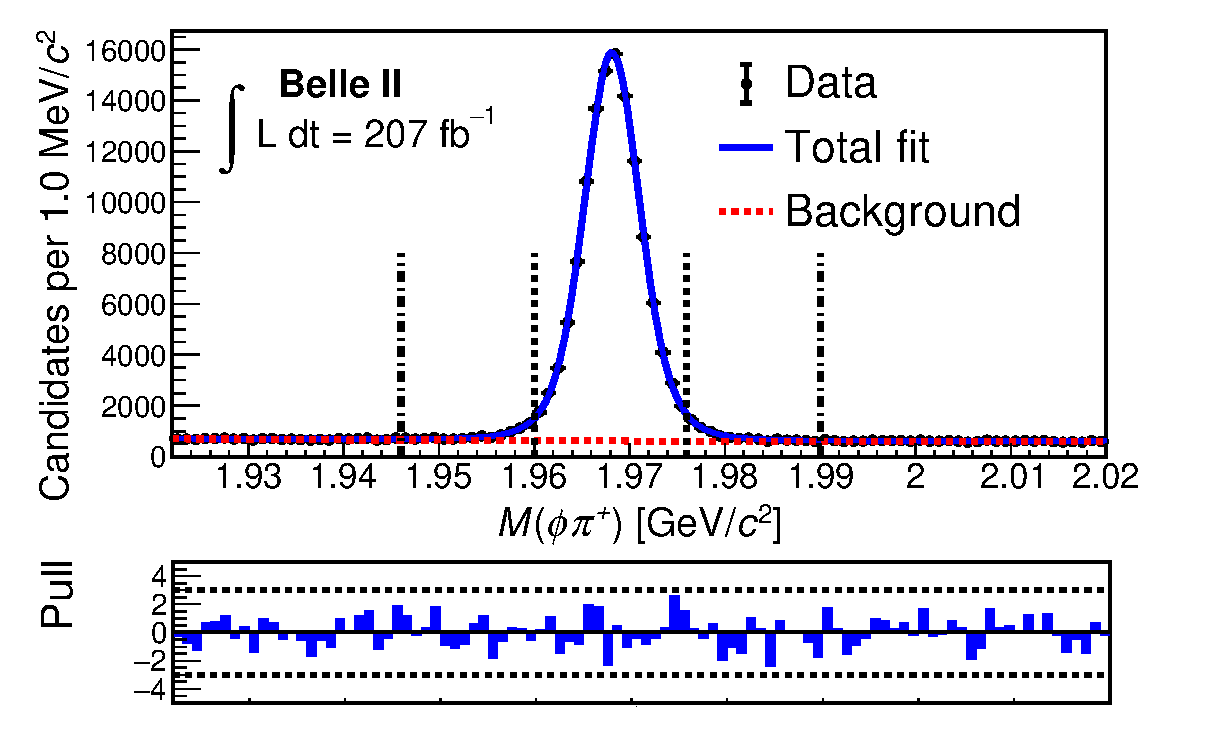
\includegraphics[width=0.50\textwidth]{c1d_dsm.eps}
    \caption{Distribution of $M(\phi\pi^+)$ for $\Dsphipi$ candidates,
        with the fit result overlaid. Black dots correspond to the data; 
       the red dashed curve shows the background component; and the blue 
       solid curve shows the overall fit result.
       Vertical dotted lines denote the signal region, and 
      vertical dot-dashed lines denote the upper and lower boundaries 
      of the lower and upper sidebands (see text). 
       The corresponding pull distribution is shown 
     in the lower panel, where the pull is defined as 
     $({\rm data}-{\rm fit})/({\rm uncertainty\ in\ data})$. }
    \label{fig:Mkkpi_plot}
\end{figure}

The decay time of a $D_s^+$ candidate is calculated as
\begin{eqnarray}
\trec & = & \left(\frac{\vec{d}\cdot\vec{p}}{p^2}\right) m^{}_{D_s^+} \,,
\label{eqn:decay_time}
\end{eqnarray}
where $\vec{d}$ is the displacement vector from the IP to the $D_s^+$
decay vertex, $\vec{p}$ is the $D_s^+$ momentum, and $m^{}_{D_s^+}$ is the
known $D_s^+$ mass~\cite{ParticleDataGroup:2022pth}.
The average resolution on $\trec$ is 108~fs.
We determine the $D^+_s$ lifetime by performing an unbinned maximum 
likelihood fit to two observables: the decay time $\trec$ and the 
per-candidate uncertainty on $\trec$ ($\sigmat$)
as calculated from the uncertainties on $\vec{d}$ and~$\vec{p}$.
The likelihood function for the $i$th candidate is given by
\begin{eqnarray} \label{eqn:likelihood_lftm}
{\cal L}(\tau | t^i,\sigmat{}\!\!^i) & = & 
f_{\rm sig}\,P_{\rm{sig}}(t^i | \tau, \sigmat{}\!\!^i)\,P_{\rm{sig}}(\sigmat{}\!\!^i)\ +\   
\nonumber \\
 & & \hskip 0.08in
(1-f_{\rm{sig}})\,P_{\rm{bkg}}(t^i|\tau, \sigmat{}\!\!^i)\,P_{\rm{bkg}}(\sigmat{}\!\!^i) ,
\end{eqnarray}
where $f^{}_{\rm sig}$ is the fraction of events that are signal $\Dsphipi$ decays;
$P_{\rm sig}(t | \sigmat)$ and $P_{\rm bkg}(t | \sigmat)$ are probability density 
functions (PDFs) for signal and background events, respectively, for a 
reconstructed decay time $\trec$ given an uncertainty $\sigmat$; 
and $P_{\rm sig}(\sigmat)$ and 
$P_{\rm bkg}(\sigmat)$ are the respective PDFs for~$\sigmat$. To reduce 
highly mismeasured events that are difficult to simulate, we impose loose 
requirements $-2000~{\rm fs}< \trec <4000$~fs and $\sigma^{}_t<900$~fs.
These requirements reject less than 0.1\% of signal candidates.


The signal PDF is the convolution of an exponential function
and a resolution function $R$:
\begin{eqnarray}
P^{}_{\rm sig}(t^i|\tau, \sigmat{}\!\!^i)  
& = & \frac{1}{\tau} \int e^{-t'/\tau}\,R(t^i-t' ; \mu, s, \sigmat{}\!\!^i)\,dt' ,
\label{lftm_pdf}
\end{eqnarray}
where $R(t^i-t' ; \mu, s, \sigmat{}\!\!^i)$ is a single Gaussian function
with mean $\mu$ and a per-candidate standard deviation $s\times \sigmat{}\!\!^i$. 
The scaling factor $s$ accounts for under- or over-estimation of the 
uncertainty $\sigmat{}\!\!^i$. The PDF $P_{\rm bkg}(t\,|\sigmat)$ is determined 
by fitting the decay-time distribution of events in the 
$M(\phi\pi^+)$ ``upper'' sideband 
$1.990~{\rm GeV}/c^2 < M(\phi\pi^+) <2.020~{\rm GeV}/c^2$,
which has no contamination from signal decays with final-state radiation.
We model $P_{\rm bkg}(t|\sigmat)$ as the sum of three asymmetric Gaussians with a common mean. 
We use MC simulation to verify that the decay-time distribution of background events in this
sideband describes well the decay-time distribution of background events in the signal region.

The PDFs $P^{}_{\rm sig}(\sigmat)$ and $P^{}_{\rm bkg}(\sigmat)$ are taken 
to be finely binned histograms. 
The former is determined from the $\sigmat$ distribution of events in the signal region, 
after subtracting the $\sigmat$ distribution of events in the $M(\phi\pi^+)$ sideband. 
The latter is determined from background events in the $M(\phi\pi^+)$ sideband.  
The resulting distribution matches well that of MC-simulated signal decays. 
The signal fraction $f_{\rm{sig}}$ is obtained from the earlier fit to the 
$M(\phi\pi^+)$ distribution (Fig.~\ref{fig:Mkkpi_plot}) and fixed in this fit.
Thus there are three floated parameters: the lifetime $\tau$, and the 
mean parameter $\mu$ and scaling factor $s$ of the resolution function. 
These are determined by maximizing the total log-likelihood
$\sum_i \ln {\cal L}(\tau | t^i,\sigmat{}\!\!^i)$, 
where the sum runs over all events in the signal region.

The result of the fit %to the events in this region 
is $\tau = 498.70 \pm 1.71$~fs, where the uncertainty is statistical only. 
The projection of the fit for $\trec$ is shown in Fig.~\ref{fig:datafit_tproj} 
along with the resulting pulls; the $\chi^2$ divided by the number of degrees 
of freedom ($100-4 = 96$) is 1.02.
The values $\mu = 0.56 \pm 0.86$~fs and $s=1.22 \pm 0.01$
obtained for the resolution function are similar to those 
obtained from MC-simulated samples.

\begin{figure}[ht]
    \centering
    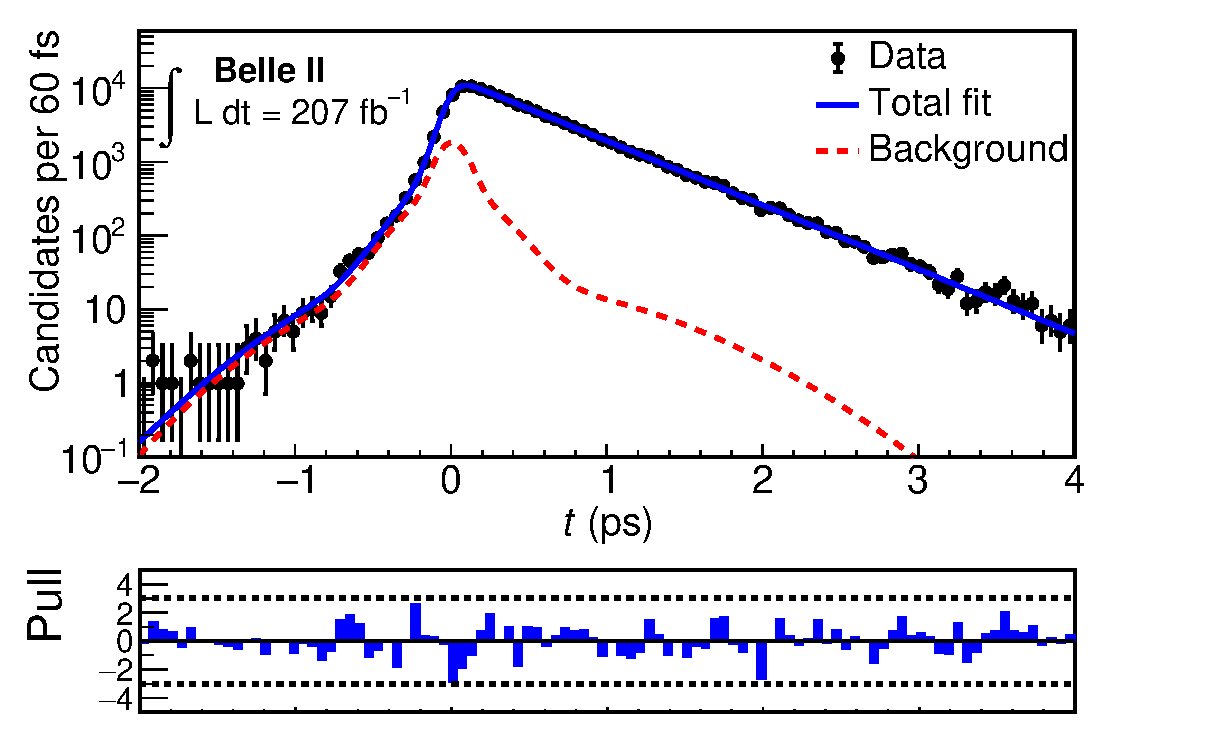
\includegraphics[scale=0.48]{fit_data_100p.eps}
    \caption{Distribution of $\trec$ for $\Dsphipi$ candidates,
        with the fit result overlaid. Black dots correspond to the data; 
       the red dashed curve shows the background component; and the blue solid 
       curve shows the overall fit result. The corresponding pull distribution 
       is shown in the lower panel.}
    \label{fig:datafit_tproj}
\end{figure}

The main systematic uncertainties are listed in 
Table~\ref{tab:syst_summary} and evaluated as follows.
Uncertainty arising
from possible mismodeling of the detector response and 
possible correlations between $\trec$ and $\sigmat$ not 
accounted for by the resolution function is assessed
by fitting a large ensemble of MC signal events. 
The mean fitted value is calculated, and the signed
difference between the mean value and the input value
is assigned as a systematic uncertainty.

There is uncertainty arising from modeling the background decay-time distribution.
We model this distribution using background events in the upper $M(\phi\pi^+)$ sideband 
$1.990~{\rm GeV}/c^2 < M(\phi\pi^+) <2.020~{\rm GeV}/c^2$. To evaluate uncertainty in this model,
we choose a lower sideband $1.922~{\rm GeV}/c^2 < M(\phi\pi^+) <1.946~{\rm GeV}/c^2$, a 
combination of the two sidebands, and also the MC-simulated background spectrum in 
the signal region.
The largest difference observed between the resulting fitted lifetime and our 
nominal result is assigned as a systematic uncertainty. 

We model both signal and background $\sigmat$ distributions using histogram PDFs, 
and there is systematic uncertainty arising from our choice for the number of bins
(i.e., statistical fluctuations of the sideband data used to obtain the histogram PDF).
We evaluate this by changing the number of bins from the nominal value (80) to 
other values in the range 60--400. For each choice of binning, we refit 
for $\tau$. The largest difference observed between the resulting values and 
our nominal value is taken as a systematic uncertainty. 

As measuring the decay time depends on a precise determination of the
displacement vector $\vec{d}$ and momentum $\vec{p}$ (Eq.~\ref{eqn:decay_time}), 
there is uncertainty arising from possible misalignments of the PXD, SVD, and 
CDC detectors. We study the effect of such possible misalignment using MC events 
reconstructed with various misalignments. Each sample is equivalent in size to that 
of the collision data used. The difference between the fitted value of $\tau$ and 
the result obtained with no misalignment is recorded, and the root-mean-square (r.m.s.) 
of the distribution of differences is taken as the systematic uncertainty due to 
possible detector misalignment. 

There is uncertainty arising from the fraction of signal candidates ($f^{}_{\rm sig}$),
which is fixed in the decay-time fit to the value obtained
from the fit to the $M(\phi\pi^+)$ distribution. We vary this parameter by 
its uncertainty and take the resulting change in the fitted lifetime as a 
systematic uncertainty. 

There is an uncertainty arising from the global momentum scale of the detector,
which is calibrated using the peak position of $D^0\ra K^-\pi^+$ decays.
We evaluate this by varying the global scale factor by its uncertainty 
($\pm 0.06\%$) and assigning the resulting variation in the fitted 
lifetime as a systematic uncertainty.

Finally, we include a systematic uncertainty due to uncertainty in the 
$D_s^+$ mass~\cite{ParticleDataGroup:2022pth}, which is used to calculate 
the decay time from the displacement vector $\vec{d}$ [see Eq.~(\ref{eqn:decay_time})].
The total systematic uncertainty is obtained by adding together all individual 
contributions (listed in Table~\ref{tab:syst_summary}) in quadrature. 
The result is $^{+1.14}_{-0.76}$~fs.

\begin{table}[ht]
\renewcommand{\arraystretch}{1.2}
\begin{tabular}{lc} 
\hline \hline
Source                                   & Uncertainty (fs)   \\ 
\hline    
Resolution function                      &   $+ 0.85$       \\
Background $(\trec,\sigma^{}_t)$ distribution  &  $\pm 0.40$       \\
Binning of $\sigmat$ histogram PDF      &   $\pm 0.10$       \\
Imperfect detector alignment             &  $\pm 0.56$       \\
Sample purity                            &   $\pm 0.09$       \\
Momentum scale factor                    &   $\pm 0.28$       \\
$D^+_s$ mass                             &   $\pm 0.02$       \\ \hline
Total                                    &   $^{+1.14}_{-0.76}$ \\ 
\hline \hline 
\end{tabular}
\caption{Summary of systematic uncertainties.}
\label{tab:syst_summary}
\end{table}


As a final check of our analysis procedure, we divide the data 
sample into subsets based on $D_s^+$ (or $D_s^-$) charge, 
$D_s^+$ momentum, $D_s^+$ polar angle, $D_s^+$ azimuthal 
angle, and data-collection (run) period, and we measure the 
lifetime separately for each subset. All measured values are 
consistent with statistical fluctuations about the overall result.
The fitted lifetime for different run periods is plotted in Fig.~\ref{fig:run_period}.

\begin{figure}[ht]
    \centering
    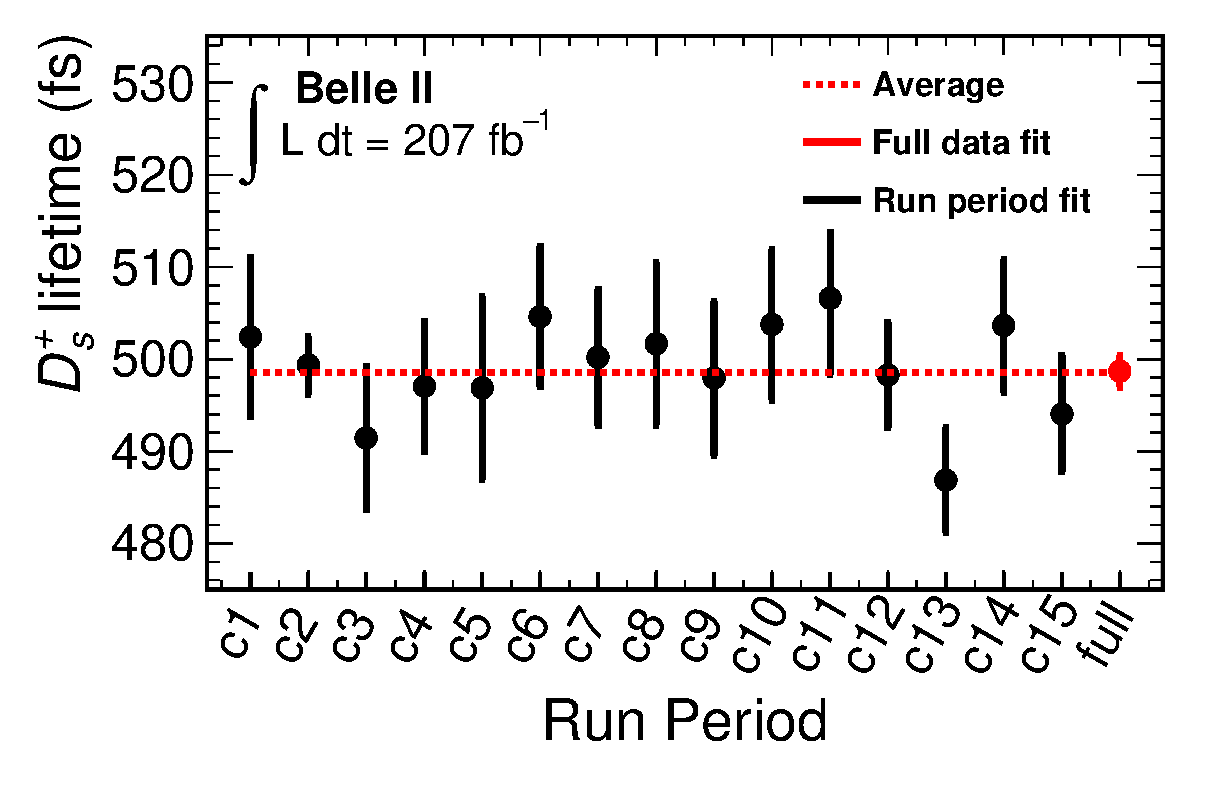
\includegraphics[scale=0.41]{exp_split_fit_res.eps}
    \caption{
    Fitted lifetime for different data-collection periods (c1--c15). 
    For these fits, the parameters of the resolution
    function are fixed to the overall fitted values.
    All values are consistent with the overall result, which is plotted 
    as a red data point. The red dashed line shows the average of the
    lifetime results for the different data-collection periods.
    }
    \label{fig:run_period}
\end{figure}

In summary, we have used $116\times 10^3$ $D_s^+\ra\phi\pi^+$ decays 
reconstructed in 207~fb$^{-1}$ of data recorded by Belle~II 
in $e^+e^-$ collisions at or near the $\Upsilon(4S)$ resonance 
to measure the $D_s^+$ lifetime. The result is
\begin{eqnarray}
\tau^{}_{D^+_s} & = & (498.7 \pm 1.7\,^{+1.1}_{-0.8})~{\rm fs,}
\end{eqnarray}
where the first uncertainty is statistical and the second is systematic. 
This is the most precise measurement to date. It is consistent with, but 
has twice the precision of, the current world-average value of 
$(504\pm 4)$~fs~\cite{ParticleDataGroup:2022pth}. It is also consistent 
with theory predictions~\cite{Lenz:2014jha, PhysRevD.88.034004,Gratrex:2022xpm}.


% Policy from October 20, 2022
This work, based on data collected using the Belle II detector, which was built and commissioned prior to March 2019, was supported by
%Armenia
Science Committee of the Republic of Armenia Grant No.~20TTCG-1C010;
%Australia
Australian Research Council and research Grants
No.~DP200101792, % Jackson
No.~DP210101900, % Urquijo
No.~DP210102831, % Sevior
No.~DE220100462, % Hsu
No.~LE210100098, % Infrastructure
and
No.~LE230100085; % Infrastructure
%Austria
Austrian Federal Ministry of Education, Science and Research,
Austrian Science Fund
No.~P~31361-N36
and
No.~J4625-N,
and
Horizon 2020 ERC Starting Grant No.~947006 ``InterLeptons'';
%Canada
Natural Sciences and Engineering Research Council of Canada, Compute Canada and CANARIE;
%China
National Key R\&D Program of China under Contract No.~2022YFA1601903,
National Natural Science Foundation of China and research Grants
No.~11575017,
No.~11761141009,
No.~11705209,
No.~11975076,
No.~12135005,
No.~12150004,
No.~12161141008,
and
No.~12175041,
and Shandong Provincial Natural Science Foundation Project~ZR2022JQ02;
%Czech Republic
the Ministry of Education, Youth, and Sports of the Czech Republic under Contract No.~LTT17020 and
Charles University Grant No.~SVV 260448 and
the Czech Science Foundation Grant No.~22-18469S;
%EU
European Research Council, Seventh Framework PIEF-GA-2013-622527,
Horizon 2020 ERC-Advanced Grants No.~267104 and No.~884719,
Horizon 2020 ERC-Consolidator Grant No.~819127,
Horizon 2020 Marie Sklodowska-Curie Grant Agreement No.~700525 "NIOBE"
and
No.~101026516,
and
Horizon 2020 Marie Sklodowska-Curie RISE project JENNIFER2 Grant Agreement No.~822070 (European grants);
%France
L'Institut National de Physique Nucl\'{e}aire et de Physique des Particules (IN2P3) du CNRS (France);
%Germany
BMBF, DFG, HGF, MPG, and AvH Foundation (Germany);
%India
Department of Atomic Energy under Project Identification No.~RTI 4002 and Department of Science and Technology (India);
%Israel
Israel Science Foundation Grant No.~2476/17,
U.S.-Israel Binational Science Foundation Grant No.~2016113, and
Israel Ministry of Science Grant No.~3-16543;
%Italy
Istituto Nazionale di Fisica Nucleare and the research grants BELLE2;
%Japan
Japan Society for the Promotion of Science, Grant-in-Aid for Scientific Research Grants
No.~16H03968,
No.~16H03993,
No.~16H06492,
No.~16K05323,
No.~17H01133,
No.~17H05405,
No.~18K03621,
No.~18H03710,
No.~18H05226,
No.~19H00682, % Niigata
No.~22H00144,
No.~26220706,
and
No.~26400255,
the National Institute of Informatics, and Science Information NETwork 5 (SINET5), 
and
the Ministry of Education, Culture, Sports, Science, and Technology (MEXT) of Japan;  
%Korea
National Research Foundation (NRF) of Korea Grants
No.~2016R1\-D1A1B\-02012900,
No.~2018R1\-A2B\-3003643,
No.~2018R1\-A6A1A\-06024970,
No.~2018R1\-D1A1B\-07047294,
No.~2019R1\-I1A3A\-01058933,
No.~2022R1\-A2C\-1003993,
and
No.~RS-2022-00197659,
Radiation Science Research Institute,
Foreign Large-size Research Facility Application Supporting project,
the Global Science Experimental Data Hub Center of the Korea Institute of Science and Technology Information
and
KREONET/GLORIAD;
%Malaysia
Universiti Malaya RU grant, Akademi Sains Malaysia, and Ministry of Education Malaysia;
%Mexico
% CINVESTAV-IPN, UNAM, UAS, BUAP and CONACYT are funded under
Frontiers of Science Program Contracts
No.~FOINS-296,
No.~CB-221329,
No.~CB-236394,
No.~CB-254409,
and
No.~CB-180023, and No.~SEP-CINVESTAV research Grant No.~237 (Mexico);
%Poland
the Polish Ministry of Science and Higher Education and the National Science Center;
%Russia
the Ministry of Science and Higher Education of the Russian Federation,
Agreement No.~14.W03.31.0026, and
the HSE University Basic Research Program, Moscow;
%Saudi Arabia
University of Tabuk research Grants
No.~S-0256-1438 and No.~S-0280-1439 (Saudi Arabia);
%Slovenia
Slovenian Research Agency and research Grants
No.~J1-9124
and
No.~P1-0135;
%Spain
Agencia Estatal de Investigacion, Spain
Grant No.~RYC2020-029875-I
and
Generalitat Valenciana, Spain
Grant No.~CIDEGENT/2018/020
%Taiwan
Ministry of Science and Technology and research Grants
No.~MOST106-2112-M-002-005-MY3
and
No.~MOST107-2119-M-002-035-MY3,
and the Ministry of Education (Taiwan);
%Thailand
Thailand Center of Excellence in Physics;
%Turkey
TUBITAK ULAKBIM (Turkey);
%Ukraine
National Research Foundation of Ukraine, project No.~2020.02/0257,
and
Ministry of Education and Science of Ukraine;
%USA
the U.S. National Science Foundation and research Grants
No.~PHY-1913789 % Indiana CEEM
and
No.~PHY-2111604, % Luther
and the U.S. Department of Energy and research Awards
No.~DE-AC06-76RLO1830, % PNNL
No.~DE-SC0007983, % Wayne State
No.~DE-SC0009824, % Florida
No.~DE-SC0009973, % VPI
No.~DE-SC0010007, % Duke
No.~DE-SC0010073, % South Carolina
No.~DE-SC0010118, % Carnegie Mellon
No.~DE-SC0010504, % Hawaii
No.~DE-SC0011784, % Cincinnati
No.~DE-SC0012704, % BNL
No.~DE-SC0019230, % Duke
No.~DE-SC0021274, % Mississippi
No.~DE-SC0022350, % Louisville
No.~DE-SC0023470; % South Alabama
%last group
and
%Vietnam
the Vietnam Academy of Science and Technology (VAST) under Grant No.~DL0000.05/21-23.

% Policy from October 20, 2022
These acknowledgements are not to be interpreted as an endorsement of any statement made
by any of our institutes, funding agencies, governments, or their representatives.

We thank the SuperKEKB team for delivering high-luminosity collisions;
the KEK cryogenics group for the efficient operation of the detector solenoid magnet;
the KEK computer group and the NII for on-site computing support and SINET6 network support;
and the raw-data centers at BNL, DESY, GridKa, IN2P3, INFN, and the University of Victoria for offsite computing support.


\bibliographystyle{apsrev}
\bibliography{references}

\end{document}
